\documentclass{article}

\usepackage{minted}
\usepackage{titlesec}
\usepackage{graphicx}
\usepackage{float}
\usepackage{mdframed}
\usepackage{xcolor}
\usepackage{xurl}
\usepackage{geometry}

\newgeometry{hmargin={17mm,17mm}}

% Prevent word break at end of line
\tolerance=1
\emergencystretch=\maxdimen
\hyphenpenalty=10000
\hbadness=10000

\title{Evaluation task for Awkward Array GSoC project}
\author{Pratyush Das$^1$}
% https://tex.stackexchange.com/a/315873/193728
\date{%
    $^1$Institute of Engineering \& Management, Kolkata\\%
}

\begin{document}

\definecolor{light-gray}{gray}{0.95}

\maketitle

\begin{abstract}

    In this report, we demonstrate a sample GPU kernel designed to be an alternative to the CPU backend for array operations in the Awkward Array project. In particular, we implement a CUDA translation of the \textit{awkward\_listarray\_compact\_offsets} CPU kernel, and show how parallelizing the code on a GPU could significantly increase the speed of computation. The motivation of this report is to serve as an evaluation to enable me to qualify to work on the project titled ``Awkward Array GPU kernels" under the mentorship of Jim Pivarski and David Lange.

\end{abstract}

\section{Introduction}

The sample CPU kernel (directly taken from the Awkward Array codebase) to be translated is defined below -
\begin{mdframed}[backgroundcolor=light-gray, roundcorner=10pt,leftmargin=0.5, rightmargin=0.5, innertopmargin=5,innerbottommargin=5, outerlinewidth=1, linecolor=light-gray]
\begin{minted}{c}
template <typename C, typename T>
ERROR awkward_listarray_compact_offsets(T* tooffsets, const C* fromstarts, const C* fromstops, 
          int64_t startsoffset, int64_t stopsoffset, int64_t length) {
  tooffsets[0] = 0;
  for (int64_t i = 0;  i < length;  i++) {
    C start = fromstarts[startsoffset + i];
    C stop = fromstops[stopsoffset + i];
    if (stop < start) {
      return failure("stops[i] < starts[i]", i, kSliceNone);
    }
    tooffsets[i + 1] = tooffsets[i] + (stop - start);
  }
  return success();
}
\end{minted}
\end{mdframed}
Translating this particular CPU kernel serves as a good test because parallelizing this CPU kernel involves overcoming the loop carried dependency in the above code -
\begin{mdframed}[backgroundcolor=light-gray, roundcorner=10pt,leftmargin=0.5, rightmargin=0.5, innertopmargin=1,innerbottommargin=1, outerlinewidth=1, linecolor=light-gray]
\begin{minted}{c}
tooffsets[i + 1] = tooffsets[i] + (stop - start);
\end{minted}
\end{mdframed}
where \mintinline{c}{tooffsets[i + 1]} depends on \mintinline{c}{toffsets[i]}.\\

\pagebreak
The above algorithm can be visualized to illustrate its linear nature -
\begin{figure}[H]
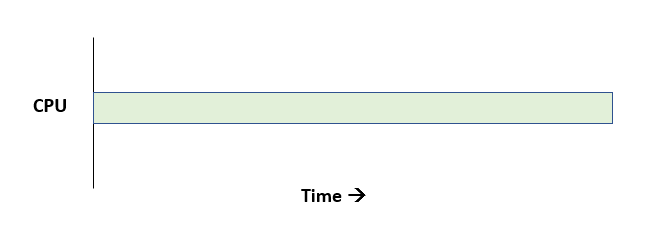
\includegraphics[width=\textwidth]{Graphics/cpu.PNG}
\caption{Visualizing sequential CPU algorithm}
\end{figure}

\subsection{Implementation of GPU algorithm}

The evaluation task required creating a parallel algorithm as an alternative for the sequential CPU algorithm. There are several ways to do this -
\begin{enumerate}
    \item OpenCL \cite{opencl}, which is a more uniform interface to write parallel algorithms to be executed on multiple backends, but is slower than CUDA and losing popularity.
    \item CUDA \cite{cuda}, which is an easier and more performant interface for executing parallel algorithms only on an NVIDIA GPU.
\end{enumerate}
Due to the availability of an NVIDIA GPU and performance requirements, we have decided to use CUDA to write and execute our parallel algorithms.
\smallbreak
\noindent We use some CUDA intrinsics like \mintinline{c}{thrust} \cite{thrust} in our sample code for the evaluation task which we might not use in the production code to avoid locking our parallel implementation to CUDA and allow expansion to newer interfaces in the future.

\section{Sequential algorithm on an Nvidia GPU}

\subsection{Sequential algorithm on a single thread}

\begin{figure}[H]
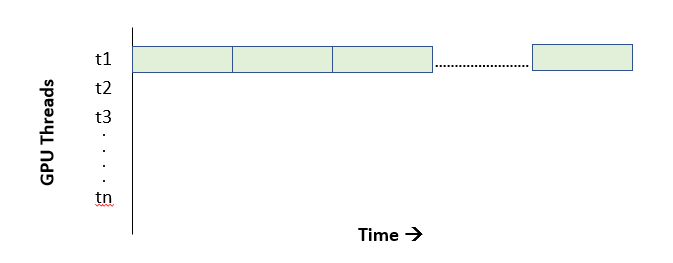
\includegraphics[width=\textwidth]{Graphics/naivesingle.PNG}
\caption{Visualizing GPU threads at work}
\end{figure}
\begin{mdframed}[backgroundcolor=light-gray, roundcorner=10pt,leftmargin=0.5, rightmargin=0.5, innertopmargin=5,innerbottommargin=5, outerlinewidth=1, linecolor=light-gray]
\begin{minted}{c}
__device__
void success_cuda(Error* err) {
  err.str = nullptr;
  err.identity = kSliceNone;
  err.attempt = kSliceNone;
  err.extra = 0;
}

__device__
void failure_cuda(const char* str, int64_t identity, int64_t attempt, Error* err) {
  err.str = str;
  err.identity = identity;
  err.attempt = attempt;
  err.extra = 0;
}

template <typename C, typename T>
__global__
void awkward_listarray_compact_offsets(T* tooffsets, const C* fromstarts, const C* fromstops, 
        int64_t startsoffset, int64_t stopsoffset, int64_t length, Error* err) {
  __shared__ int flag[1];
  int idx = threadIdx.x + (blockIdx.x * blockDim.x);
  if (idx == 0) {
    tooffsets[0] = 0;
    flag[0] = 0;
  }
  if (idx < length) {
    if (idx == 0) {
      for (int i = 0; i < length; i++) {
        C start = fromstarts[startsoffset + i];
        C stop = fromstops[stopsoffset + i];
        if (stop < start) {
          failure_cuda("stops[i] < starts[i]", i, kSliceNone, err);
          flag[0] = 1;
        }
        tooffsets[i + 1] = tooffsets[i] + (stop - start);
      }
    }
  }
  __syncthreads();
  if (flag[0] != 1) {
    success_cuda(err);
  }
}
\end{minted}
\end{mdframed}
In the above code block\footnote{Full benchmarking code: \url{https://github.com/reikdas/GSoC-Proposal-2020/blob/master/testgsoc/naivesingle.cu}} we execute the algorithm only for a single GPU thread (in a for loop) while the other threads sit idle.
\begin{mdframed}[backgroundcolor=light-gray, roundcorner=10pt,leftmargin=0.5, rightmargin=0.5, innertopmargin=1,innerbottommargin=1, outerlinewidth=1, linecolor=light-gray]
\begin{minted}{c}
    if (idx == 0) {
        ...
    }
\end{minted}
\end{mdframed}
where the variable \mintinline{c}{idx} is the thread index.\\
\\
Since CUDA GPU kernels have to be of the return type void, we use additional device functions, \mintinline{c}{success_cuda} and \mintinline{c}{failure_cuda} to record whether the kernel behaved as expected.\\
\begin{mdframed}[backgroundcolor=light-gray, roundcorner=10pt,leftmargin=0.5, rightmargin=0.5, innertopmargin=5,innerbottommargin=5, outerlinewidth=1, linecolor=light-gray]
\begin{minted}{c}
__device__
void success_cuda(Error* err) {
  err.str = nullptr;
  err.identity = kSliceNone;
  err.attempt = kSliceNone;
  err.extra = 0;
}

__device__
void failure_cuda(const char* str, int64_t identity, 
                  int64_t attempt, Error* err) {
  err.str = str;
  err.identity = identity;
  err.attempt = attempt;
  err.extra = 0;
}
\end{minted}
\end{mdframed}
We use a flag which has been implemented using shared memory and the CUDA intrinsic thread synchronization 
\begin{mdframed}[backgroundcolor=light-gray, roundcorner=10pt,leftmargin=0.5, rightmargin=0.5, innertopmargin=5,innerbottommargin=5, outerlinewidth=1, linecolor=light-gray]
\begin{minted}{c}
    __shared__ int flag[1];
    ...
    __syncthreads();
    if (flag[0] != 1) {
        ...
    }
\end{minted}
\end{mdframed}
to determine whether the \mintinline{c}{success_cuda()} call should be executed once the \mintinline{c}{failure_cuda()} call has already been reached by one of the GPU threads.

\subsection{Sequential algorithm on multiple threads}

\begin{figure}[H]
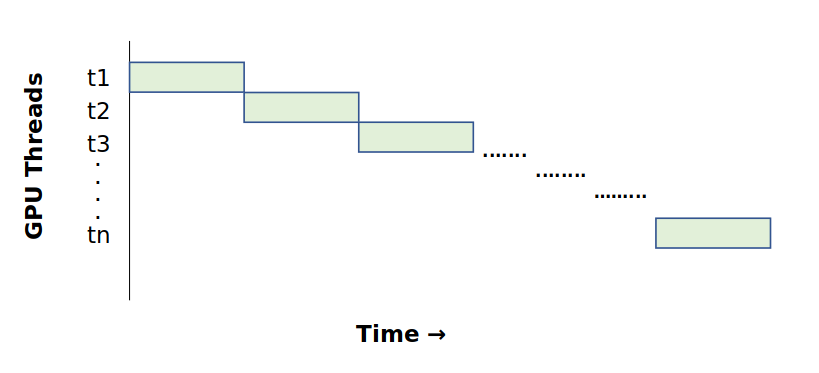
\includegraphics[width=\textwidth]{Graphics/naivemulti.PNG}
\caption{Visualizing GPU threads at work}
\end{figure}
\begin{mdframed}[backgroundcolor=light-gray, roundcorner=10pt,leftmargin=0.5, rightmargin=0.5, innertopmargin=5,innerbottommargin=5, outerlinewidth=1, linecolor=light-gray]
\begin{minted}{c}
__device__
void success_cuda(Error* err) {
  err.str = nullptr;
  err.identity = kSliceNone;
  err.attempt = kSliceNone;
  err.extra = 0;
}

__device__
void failure_cuda(const char* str, int64_t identity, int64_t attempt, Error* err) {
  err.str = str;
  err.identity = identity;
  err.attempt = attempt;
  err.extra = 0;
}

template <typename C, typename T>
__global__
void awkward_listarray_compact_offsets(T* tooffsets, const C* fromstarts, const C* fromstops, 
        int64_t startsoffset, int64_t stopsoffset, int64_t length, Error* err) {
  __shared__ int flag[1];
  int idx = threadIdx.x + (blockIdx.x * blockDim.x);
  if (idx < length) {
    if (idx == 0) {
      tooffsets[0] = 0;
      flag[0] = 0;
    }
    for (int i = 0; i < length; i++) {
      __syncthreads();
      if (i == idx) {
        C start = fromstarts[startsoffset + i];
        C stop = fromstops[stopsoffset + i];
        if (stop < start) {
          failure_cuda("stops[i] < starts[i]", i, kSliceNone, err);
          flag[0] = 1;
        }
        tooffsets[i + 1] = tooffsets[i] + (stop - start);
      }
    }
  }
  __syncthreads();
  if (flag[0] != 1) {
    success_cuda(err);
  }
}

\end{minted}
\end{mdframed}
The sequential algorithm on multiple GPU threads implementation shown above\footnote{Full benchmarking code: \url{https://github.com/reikdas/GSoC-Proposal-2020/blob/master/testgsoc/naivemultiblocks.cu}} differs only slightly from the sequential algorithm on a single GPU thread implementation.
\smallbreak
\noindent The main difference is that the multiple GPU threads implementation has all the threads execute the algorithm one after another (no loops), instead of all at the same time. When one thread is being executed, the other threads sit idly, then the next thread is executed while the previous and all other threads sit idle.
\begin{mdframed}[backgroundcolor=light-gray, roundcorner=10pt,leftmargin=0.5, rightmargin=0.5, innertopmargin=5,innerbottommargin=5, outerlinewidth=1, linecolor=light-gray]
\begin{minted}{c}
    for (int i = 0; i < length; i++) {
      ...
      if (i == idx) {
        ... 
        }
    }
\end{minted}
\end{mdframed}
We use the CUDA intrinsic \mintinline{c}{__syncthreads()} before each iteration of the loop to ensure that all the threads are at the same position and ready to be executed before each thread is executed.

\section{Parallel algorithm on an Nvidia GPU}

\begin{figure}[H]
\hfill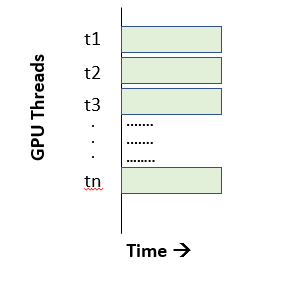
\includegraphics[scale=0.72]{Graphics/gpu.PNG}\hspace*{\fill}
\caption{Visualizing GPU threads at work}
\end{figure}
\subsection{Using Thrust}
\begin{mdframed}[backgroundcolor=light-gray, roundcorner=10pt,leftmargin=0.5, rightmargin=0.5, innertopmargin=5,innerbottommargin=5, outerlinewidth=1, linecolor=light-gray]
\begin{minted}{c}
#include <thrust/device_vector.h>
#include <thrust/scan.h>
#include "helper_cuda.h"

__device__
void success_cuda(Error* err) {
  err.str = nullptr;
  err.identity = kSliceNone;
  err.attempt = kSliceNone;
  err.extra = 0;
}

__device__
void failure_cuda(const char* str, int64_t identity, int64_t attempt, Error* err) {
  err.str = str;
  err.identity = identity;
  err.attempt = attempt;
  err.extra = 0;
}

template <typename T, typename C>
__global__
void sub(T* output, const C* starter, const C* stopper, int64_t startsoffset, 
        int64_t stopsoffset, int64_t n, Error* err) {
  __shared__ int flag[1];
  int thid = threadIdx.x + blockIdx.x * blockDim.x;
  if (thid == 0) flag[0] = 0;
  if (thid < n) {
    C start = starter[thid + startsoffset];
    C stop = stopper[thid + stopsoffset];
    if (stop < start) {
      failure_cuda("stops[i] < starts[i]", thid , kSliceNone, err);
      flag[0] = 1;
    }
    output[thid] = stop - start;
  }
  __syncthreads();
  if (flag[0] != 1) {
    success_cuda(err);
  }
}

template <typename T, typename C>
void prefix_sum(T* output, const C* arr, const C* arr2, int64_t startsoffset, 
        int64_t stopsoffset, int64_t length, Error* err) {
  int block, thread;
  if (length > 1024) {
    block = (length / 1024) + 1;
    thread = 1024;
  }
  else {
    thread = length;
    block = 1;
  }
  T* d_output;
  C* d_arr, * d_arr2;
  checkCudaErrors(cudaMalloc((void**)&d_output, length * sizeof(T)));
  checkCudaErrors(cudaMalloc((void**)&d_arr, length * sizeof(C)));
  checkCudaErrors(cudaMemcpy(d_arr, arr, length * sizeof(C), cudaMemcpyHostToDevice));
  checkCudaErrors(cudaMalloc((void**)&d_arr2, length * sizeof(C)));
  checkCudaErrors(cudaMemcpy(d_arr2, arr2, length * sizeof(C), cudaMemcpyHostToDevice));
  sub<T, C><<<block, thread>>>(d_output, d_arr, d_arr2, startsoffset, stopsoffset, length, err);
  checkCudaErrors(cudaDeviceSynchronize());
  thrust::device_vector<T> data(d_output, d_output+length);
  thrust::device_vector<T> temp(data.size() + 1);
  thrust::exclusive_scan(data.begin(), data.end(), temp.begin());
  temp[data.size()] = data.back() + temp[data.size() - 1];
  thrust::copy(temp.begin(), temp.end(), output);
  checkCudaErrors(cudaFree(d_output));
  checkCudaErrors(cudaFree(d_arr));
  checkCudaErrors(cudaFree(d_arr2));
}
\end{minted}
\end{mdframed}
The above code\footnote{Full benchmarking code: \url{https://github.com/reikdas/GSoC-Proposal-2020/blob/master/testgsoc/thrust.cu}} is the final resulting code for the evaluation task. We implement the given CPU algorithm as a parallel GPU algorithm using CUDA.\\
\noindent The CUDA kernel \mintinline{c}{sub} takes two arrays that reside on the GPU and returns a GPU array which stores the result of subtracting the value of the array at the position (indices + offset). We call \mintinline{c}{sub} from the function \mintinline{c}{prefix_sum} which also calls Thrust's exclusive scan \cite{scan} algorithm on the resulting device array to get the required result.
\begin{mdframed}[backgroundcolor=light-gray, roundcorner=10pt,leftmargin=0.5, rightmargin=0.5, innertopmargin=5,innerbottommargin=5, outerlinewidth=1, linecolor=light-gray]
\begin{minted}{c}
    thrust::exclusive_scan(data.begin(), data.end(), temp.begin());
\end{minted}
\end{mdframed}
and since the problem in question is not exactly an exclusive scan where the last cumulative sum number is not calculated, we need an additional step to calculate the required result -
\begin{mdframed}[backgroundcolor=light-gray, roundcorner=10pt,leftmargin=0.5, rightmargin=0.5, innertopmargin=5,innerbottommargin=5, outerlinewidth=1, linecolor=light-gray]
\begin{minted}{c}
    temp[data.size()] = data.back() + temp[data.size() - 1];
\end{minted}
\end{mdframed}
\noindent We calculate the number of blocks and threads required by the \mintinline{c}{sub} CUDA kernel by - 
\begin{mdframed}[backgroundcolor=light-gray, roundcorner=10pt,leftmargin=0.5, rightmargin=0.5, innertopmargin=5,innerbottommargin=5, outerlinewidth=1, linecolor=light-gray]
\begin{minted}{c}
    if (length > 1024) {
        block = (length / 1024) + 1;
        thread = 1024;
    }
    else {
        thread = length;
        block = 1;
    }
\end{minted}
\end{mdframed}
The prefix\_sum() function also has a lot of boilerplate code such as copying arrays from CPU to GPU, and back from the GPU to CPU whose execution time we do not take into consideration while benchmarking.\\
\smallbreak
\noindent Arguably CUB's \cite{cub} exclusive scan algorithm is more optimized than Thrust's exclusive scan algorithm, but since Thrust comes installed with the CUDA development toolkit, we have decided to use Thrust in our sample code.

\subsection{Implementing by hand}

Instead of using a library (for eg. Thrust) which comes with a prefix sum algorithm, in this example we implement a Hillis Steele algorithm ourselves - 

\begin{mdframed}[backgroundcolor=light-gray, roundcorner=10pt,leftmargin=0.5, rightmargin=0.5, innertopmargin=5,innerbottommargin=5, outerlinewidth=1, linecolor=light-gray]
\begin{minted}{c}
#include <cuda_runtime.h>
#include "device_launch_parameters.h"
#include <iostream>

// https://stackoverflow.com/a/14038590/4647107
#define gpuErrchk(ans) { gpuAssert((ans), __FILE__, __LINE__); }
inline void gpuAssert(cudaError_t code, const char *file, int line, bool abort=true)
{
  if (code != cudaSuccess)
  {
    fprintf(stderr,"GPUassert: %s %s %d\n", cudaGetErrorString(code), file, line);
    if (abort) exit(code);
  }
}

template <typename T, typename C>
__global__
void prefix_sum1(T* base, const C* basestart, const C* basestop, int64_t basestartoffset,
                 int64_t basestopoffset, int length, T* sums) {
  int thid = threadIdx.x + (blockIdx.x * blockDim.x);
  extern __shared__ T temp[];
  int pout = 0, pin = 1;
  if (thid < length) {
    if (thid == 0) {
      temp[threadIdx.x] = 0;
    }
    else {
      temp[threadIdx.x] = basestop[basestopoffset + thid - 1] - 
                          basestart[basestartoffset + thid - 1];
    }
    __syncthreads();
    for (int offset = 1; offset < 1024; offset *=2) {
      pout = 1 - pout;
      pin = 1 - pout;
      if (threadIdx.x >= offset) {
        temp[pout*1024 + threadIdx.x] = temp[pin*1024 + threadIdx.x - offset] + 
                                        temp[pin*1024 + threadIdx.x];
      }
      else {
        temp[pout*1024 + threadIdx.x] = temp[pin*1024 + threadIdx.x];
      }
      __syncthreads();
    }
    base[thid] = temp[pout*1024 + threadIdx.x];
    __syncthreads();
    if ((thid == 1023) || ((blockIdx.x != 0) && (thid == ((1024 * (blockIdx.x + 1))-1))) || 
        (thid == length-1)) {
        sums[blockIdx.x] = base[thid];
    }
  }
}

// Need another kernel because of conditional __syncthreads()
template <typename T>
__global__
void prefix_sum2(T* base, int length) {
  int thid = threadIdx.x + (blockIdx.x * blockDim.x);
  extern __shared__ T temp[];
  int pout = 0, pin = 1;
  if (thid < length) {
    temp[thid] = base[thid];
    __syncthreads();
    for (int offset = 1; offset < length; offset *=2) {
      pout = 1 - pout;
      pin = 1 - pout;
      if (thid >= offset)
        temp[pout*length + thid] = temp[pin*length + thid - offset] + temp[pin*length + thid];
      else
        temp[pout*length + thid] = temp[pin*length + thid];
      __syncthreads();
    }
    base[thid] = temp[pout*length + thid];
  }
}

template<typename T>
__global__
void adder(T* base, T* sums, int64_t length) {
  int thid = threadIdx.x + (blockIdx.x * blockDim.x);
  if (blockIdx.x != 0 && thid < length)
    base[thid] += sums[blockIdx.x - 1];
}

template <typename T, typename C>
void offload(T* base, C* basestart1, C* basestop1, int64_t basestartoffset, 
             int64_t basestopoffset, int64_t length) {
  int block, thread=1024;
  if (length > 1024) {
    if (length%1024 != 0)
      block = (length / 1024) + 1;
    else
      block = length/1024;
  }
  else {
    block = 1;
  }
  int modlength = block*thread;
  // Padding the input arrays
  C basestart[modlength], basestop[modlength];
  for (int i=0; i<modlength; i++) {
    if (i<length){
      basestart[i] = basestart1[i];
      basestop[i] = basestop1[i];
    }
    else {
      basestart[i] = 0;
      basestop[i] = 0;
    }
  }
  T* d_tooffsets, * d_sums;
  C* d_fromstarts, * d_fromstops;
  gpuErrchk(cudaMalloc((void**)&d_tooffsets, (modlength+1) * sizeof(T)));
  gpuErrchk(cudaMalloc((void**)&d_fromstarts, modlength * sizeof(C)));
  gpuErrchk(cudaMemcpy(d_fromstarts, basestart, modlength * sizeof(C), cudaMemcpyHostToDevice));
  gpuErrchk(cudaMalloc((void**)&d_fromstops, modlength * sizeof(C)));
  gpuErrchk(cudaMemcpy(d_fromstops, basestop, modlength * sizeof(C), cudaMemcpyHostToDevice));
  gpuErrchk(cudaMalloc((void**)&d_sums, block*sizeof(T)));
  prefix_sum1<T, C><<<block, thread, thread*2*sizeof(T)>>>(d_tooffsets, d_fromstarts, 
                     d_fromstops, basestartoffset, basestopoffset, modlength, d_sums);
  gpuErrchk(cudaPeekAtLastError());
  gpuErrchk(cudaDeviceSynchronize());
  prefix_sum2<T><<<1, block, block*2*sizeof(T)>>>(d_sums, block);
  gpuErrchk(cudaPeekAtLastError());
  gpuErrchk(cudaDeviceSynchronize());
  adder<T><<<block, thread>>>(d_tooffsets, d_sums, modlength);
  gpuErrchk(cudaPeekAtLastError());
  gpuErrchk(cudaDeviceSynchronize());
  gpuErrchk(cudaMemcpy(base, d_tooffsets, (length + 1) * sizeof(T), cudaMemcpyDeviceToHost));
  base[length] = base[length - 1] + basestop[length - 1 + basestopoffset] - 
                 basestart[length - 1 + basestartoffset];
  gpuErrchk(cudaFree(d_tooffsets));
  gpuErrchk(cudaFree(d_fromstarts));
  gpuErrchk(cudaFree(d_fromstops));
  gpuErrchk(cudaFree(d_sums));
}
\end{minted}
\end{mdframed}

Examining the algorithm in the code display above, the main complexity of this algorithm is extending the algorithm for multiple blocks. This is why we had to implement another kernel to calculate the prefix sum of an array storing the element at the last index of each block.

\begin{mdframed}[backgroundcolor=light-gray, roundcorner=10pt,leftmargin=0.5, rightmargin=0.5, innertopmargin=5,innerbottommargin=5, outerlinewidth=1, linecolor=light-gray]
\begin{minted}{c}
// Need another kernel because of conditional __syncthreads()
template <typename T>
__global__
void prefix_sum2(T* base, int length) {
  int thid = threadIdx.x + (blockIdx.x * blockDim.x);
  extern __shared__ T temp[];
  int pout = 0, pin = 1;
  if (thid < length) {
    temp[thid] = base[thid];
    __syncthreads();
    for (int offset = 1; offset < length; offset *=2) {
      pout = 1 - pout;
      pin = 1 - pout;
      if (thid >= offset)
        temp[pout*length + thid] = temp[pin*length + thid - offset] + temp[pin*length + thid];
      else
        temp[pout*length + thid] = temp[pin*length + thid];
      __syncthreads();
    }
    base[thid] = temp[pout*length + thid];
  }
}
\end{minted}
\end{mdframed}

and then add the calculated values to all the elements in the next block - 

\begin{mdframed}[backgroundcolor=light-gray, roundcorner=10pt,leftmargin=0.5, rightmargin=0.5, innertopmargin=5,innerbottommargin=5, outerlinewidth=1, linecolor=light-gray]
\begin{minted}{c}
template<typename T>
__global__
void adder(T* base, T* sums, int64_t length) {
  int thid = threadIdx.x + (blockIdx.x * blockDim.x);
  if (blockIdx.x != 0 && thid < length)
    base[thid] += sums[blockIdx.x - 1];
}
\end{minted}
\end{mdframed}

\section{Verifying results}
It is important to verify the results, especially in the case of the GPU implementations because of race conditions at the CUDA block boundaries. CUDA blocks cannot communicate with each other without the use of CUDA's cooperative groups that have been introduced since CUDA 9.\par
The GPU and CPU results have been verified by checking the results for small arrays (size < 100) by eye. The results of larger arrays have been verified by using a for loop(we do not care about speed during verification) to iterate over and compare the resulting arrays of the CPU and GPU implementations.\footnote{\url{https://github.com/reikdas/GSoC-Proposal-2020/blob/master/testgsoc/thrustcputime.cu#L90}}

\pagebreak
\section{Benchmarks}
We have compared the performance of the various algorithms relative to each other\footnote{Benchmarking numbers: \url{https://github.com/reikdas/GSoC-Proposal-2020/blob/master/testgsoc/data.txt} generated using \url{https://github.com/reikdas/GSoC-Proposal-2020/blob/master/testgsoc/plotter.py}}.
\begin{figure}[H]
\hfill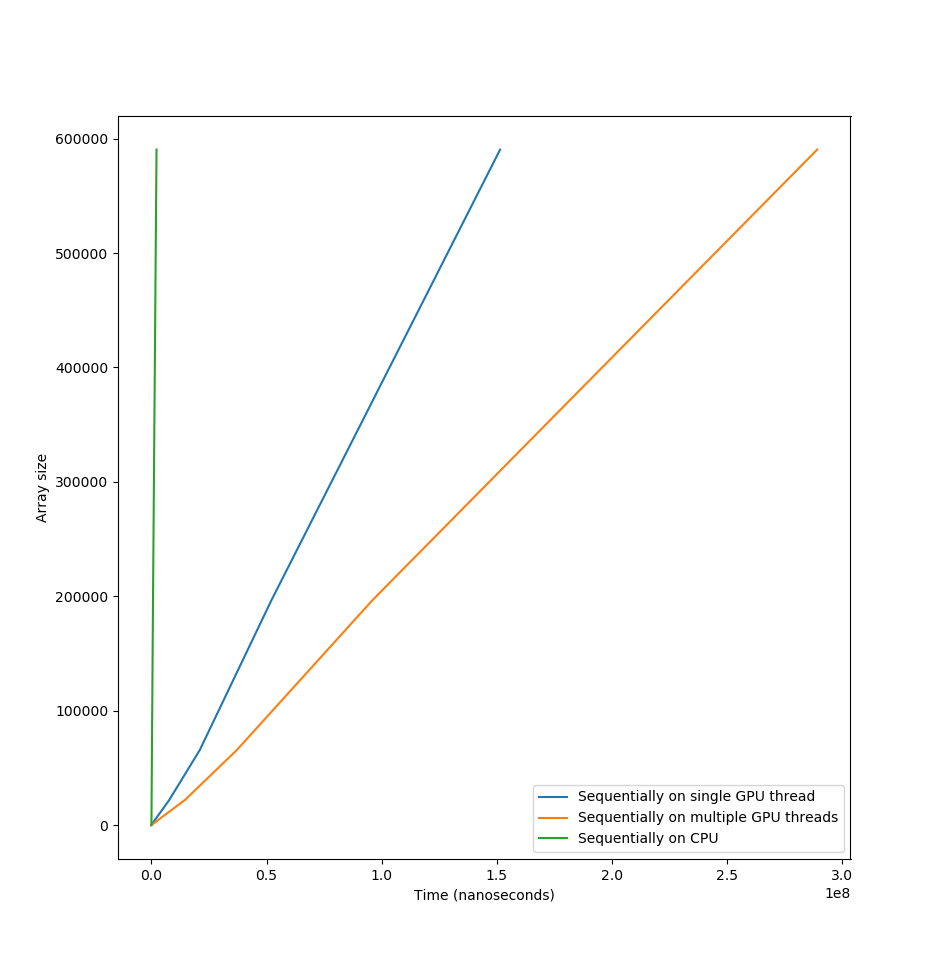
\includegraphics[scale=0.5]{Graphics/naivegpucpu.png}\hspace*{\fill}
\caption{Comparing performance of sequential GPU algorithms with CPU algorithm}
\end{figure}
We can see that the sequential algorithms on the GPU run much slower than the sequential algorithm on the CPU\footnote{We use an i7 8750H CPU for our tests}. This can be attributed to the inherent difference in the design of GPUs and CPUs. GPUs are designed to operate on independent data in parallel, whereas CPUs are optimized to execute a single stream of instructions as quickly as possible. So when we are executing a single instruction stream on the GPU, it is expected that the time for completion will be more than the time for completion of the same instructions on a CPU.

\begin{figure}[H]
\hfill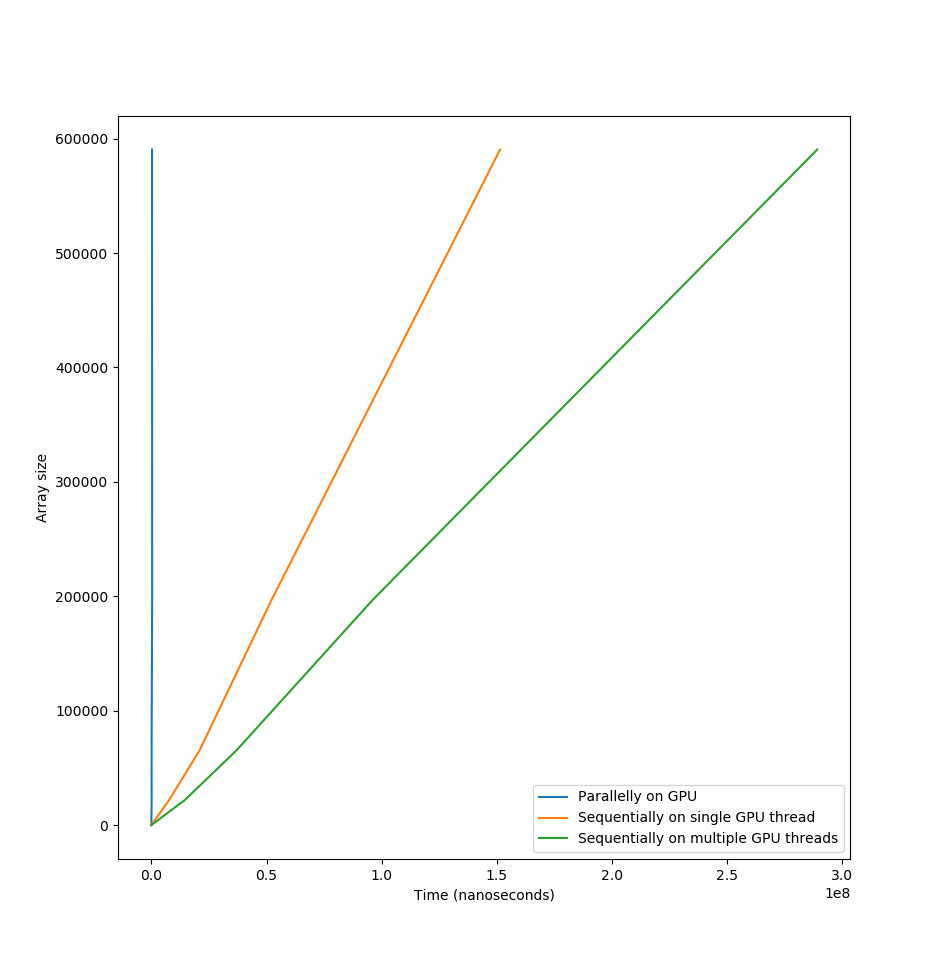
\includegraphics[scale=0.5]{Graphics/gpucomp.png}\hspace*{\fill}
\caption{Comparing performance of sequential and parallel GPU algorithms}
\end{figure}
Similar to the previous plot, we can see that our parallelized GPU implementation is much faster than the implementation of our sequential algorithms on the GPU. This gives us an indication that our parallel implementation is correct and gives a clear speedup over the sequential algorithm when executed on the same hardware (GPU of our test machine in this case)\footnote{We used an Nvidia GeForce 1070 Max Q GPU for our tests}.

\begin{figure}[H]
\hfill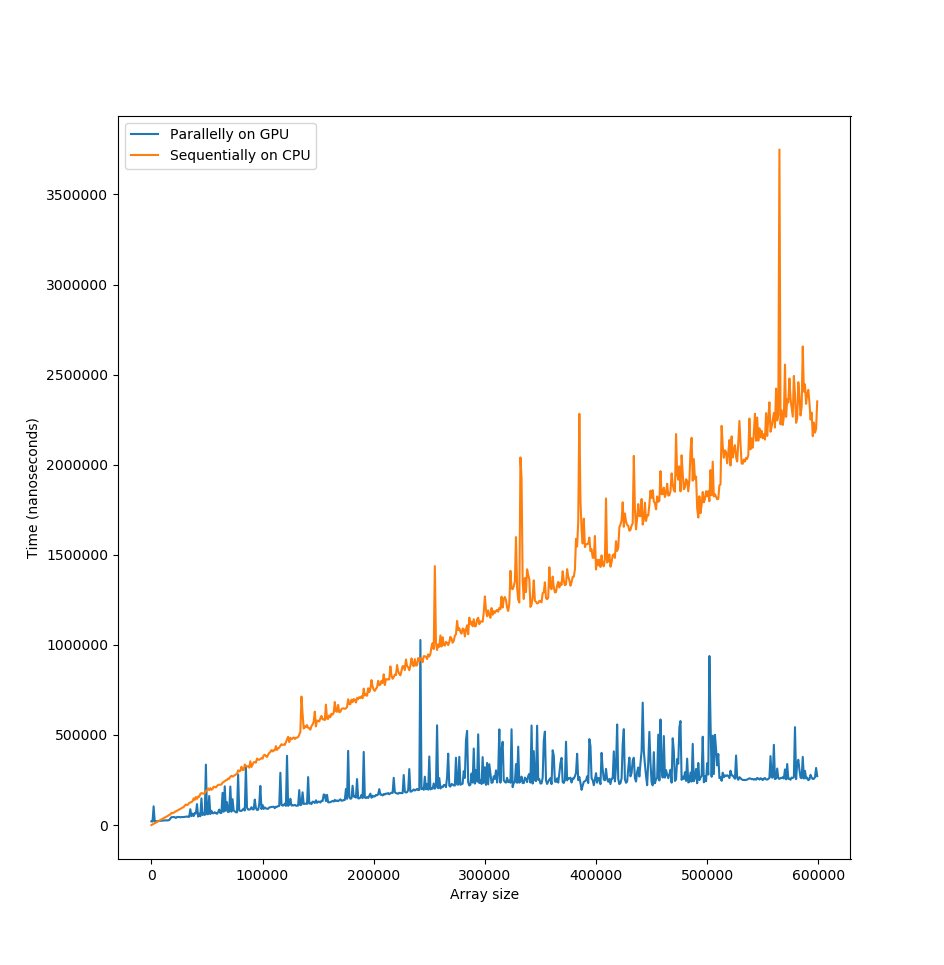
\includegraphics[scale=0.5]{Graphics/gpuvcpu.png}\hspace*{\fill}
\caption{Comparing parallelized GPU performance vs CPU performance}
\end{figure}
This is the most important result of the evaluation task. Here, we can clearly visualize that the parallel algorithm we designed to be executed on the GPU is much faster than the given sequential algorithm on the CPU.\footnote{There are some non-uniform anamolous spikes in all iterations of recorded data}

\begin{figure}[H]
\hfill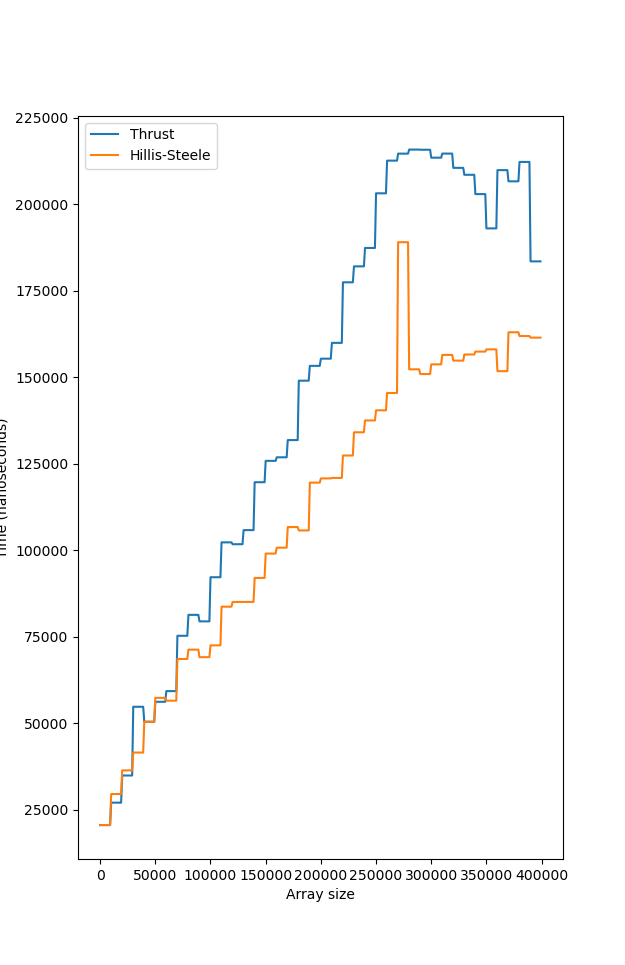
\includegraphics[scale=0.5]{Graphics/thrusthillis.png}\hspace*{\fill}
\caption{Comparing performance of Thrust vs algorithm implemented by hand(min of sliding window with 10 entries)}
\end{figure}
The above plot demonstrates that our hand written Hillis Steele algorithm is as fast as (if not faster) than the algorithm in the Thrust library. This is an important result because this means that we can extend our Hillis Steele implementation to multiple kernels with slight modifications.

\section{Appendix}
We have only demonstrated the relevant CUDA kernels and not the surrounding code or main functions which are required to execute the kernels. The entire collection of complete code samples can be found in the GitHub repository.\par
In our full sample code which we have used for benchmarking, we have used 2 header files which includes helper functions to facilitate CUDA error checking in our code - \textit{helper\_cuda.h} and \textit{helper\_string.h}. Both of these helper header files are included in the NVIDIA CUDA SDK under the \textit{samples/inc/} folder. In the Awkward Array production code we might use the same CUDA error checking header files or we might decide to write our own CUDA error checking code.

\bibliographystyle{unsrt}
\bibliography{report.bib}

\end{document}
